\chapter{Entraînement et évaluation d'un réseau de neurones}\label{ch:ent_test_valid}

Dans ce chapitre, nous traiterons des moyens généraux d'entraîner un réseau de neurones de manière supervisée, ainsi que des méthodes de l'évaluer en vue de l'améliorer.

\section{Entraînement}
L'\emph{entraînement} d'un réseau de neurones, est une phase durant laquelle on force le réseau à changer les poids et biais de ses neurones pour produire la sortie voulue pour des exemples connus; on espère ainsi que le réseau sera capable de produire la bonne sortie pour des instances encore inconnues, c'est-à-dire bien généraliser.

\subsection{Fonction objectif}
Une manière classique de suivre l'évolution du système qui apprend est de calculer un indicateur de sa performance. En l'occurrence, il s'agit d'évaluer sa performance sur le jeu de données qui lui est soumis lors de la phase d'entraînement. Le moyen le plus répandu est de calculer cet indicateur sur chacune des instances d'entraînement \(x_i\) et d'en prendre la moyenne sur l'ensemble des \(m\) instances. On appelle cet indicateur \emph{fonction de coût}, \emph{fonction de perte} ou encore \emph{fonction objectif} (\emph{cost function} ou \emph{loss function} en anglais). Pour un réseau de neurones, on définit souvent une des fonctions de coût suivantes :

\begin{align}
\kappa &= \frac{1}{m}\sum_{i = 1}^m (y_i - \hat{y}_i)^2\\
\kappa &= - \frac{1}{m}\sum_{i = 1}^m y_i \ln{\hat{y}_i} + (1 - y_i)\ln{(1 - \hat{y}_i)}
\end{align}
où : \(m\) est le nombre d'observations ; les \(y_i\) sont les réponses attendues et \(\hat{y}_i\) sont les réponses inférées par le réseau. La première fonction est appelée "erreur quadratique moyenne", la seconde "entropie croisée".

Maximiser la performance du réseau est équivalent à minimiser la fonction de coût, mais le formuler ainsi permet de profiter des techniques d'optimisation déjà existantes. On en traite dans la section suivante.

La dépendance entre la fonction de coût et les réponses \(y_i\) et \(\hat{y}_i\) est implicite. En effet, on ne peut pas les modifier directement. D'une part, $y$ n'est pas un paramètre du modèle mais une caractéristique des données, et d'autre part, $\hat{y}$ est issu d'un calcul complexe effectué à partir des données d'entrée ainsi que des poids et biais du réseau de neurones. Il serait donc plus judicieux d'expliciter la relation entre paramètres du modèle, les valeurs d'entrée et la sortie qu'il produit : 
\[ \kappa = \kappa(\boldsymbol{w}, \boldsymbol{b}, \boldsymbol{x}, \boldsymbol{y})\]
%\[ \kappa = \kappa((\dotsc, w_i, \dotsc), (\dotsc, b_i, \dotsc), (\dotsc, x_i, \dotsc), (\dotsc, y_i, \dotsc))\]
où les variables sont les regroupements des poids (respectivement des biais, entrées et réponses attendues) sous forme de vecteurs.
Cette représentation est utile pour l'algorithme qui suit.

\subsection{Descente de gradient}\label{subseq:desc_grad}
La \emph{descente de gradient} est une méthode d'optimisation très générale. Elle permet de minimiser une fonction, donc de maximiser son opposé, par étapes successives. Un point caractéristique de la méthode est qu'elle ne garantit, à condition que la fonction soit bien choisie, que la découverte d'un extremum local. De manière générale, la découverte du extremum global d'une fonction continue, s'il existe, est un problème difficile.

Bien évidemment, puisqu'il s'agit de minimiser la fonction de coût, ses propriétés vont grandement influer sur le déroulement de l'algorithme. Le cas le plus intéressant est celui d'une fonction convexe, ce qui nous assurerait que la fonction possède au plus un minimum. Si ce n'était pas le cas, la descente de gradient pourrait s'arrêter dans un minimum local loin de l'optimum global. Mais il n'est pas toujours évident de garantir cette propriété, encore moins en dimension 2 ou supérieure.

L'idée de l'algorithme de la descente de gradient est qu'à chaque itération on ajuste les paramètres de la fonction de coût, de sorte que les nouvelles valeurs renvoient une sortie plus faible qu'à l'itération précédente. On choisit de s'arrêter lorsque les variations inter-étapes sont plus faibles qu'un seuil choisi, ou lorsqu'on a effectué un certain nombre d'itérations. 

Nous avons évoqué les fonctions convexes, mais une condition nécessaire est en fait la différentiabilité de la fonction de coût. Lorsque c'est le cas, on peut associer un gradient à chaque point de cette fonction. Le gradient est un vecteur dont le sens indique la plus forte pente au voisinage du point où il est calculé. Ses coordonnées, en même nombre que les arguments de la fonction de coût, donnent directement la marche à suivre : leur signe indique comment faire varier les paramètres, et leur valeur indique de combien les changer.  

L'algorithme, incroyablement simple, est le suivant :

\begin{algorithm}
\caption{Descente de gradient}
\label{alg:desc_grad}
\begin{algorithmic}
\State  \(\boldsymbol{x} \gets \mathit{rand()}\) \Comment{Initialisation aléatoire}
\Repeat
	\State \(\boldsymbol{x} \gets \boldsymbol{x} - \eta \cdot \boldsymbol{\nabla} \kappa\)
\Until{\(\norm{\boldsymbol{\nabla} \kappa} \leq \varepsilon\)}
\end{algorithmic}
\end{algorithm}
où : \(\eta\) est un facteur appelé \emph{taux d'apprentissage}. On parle d'\emph{hyperparamètre} dans ce cas, car il n'est pas mis à jour durant l'apprentissage mais durant une phase ultérieure\footnote{En réalité, il pourrait être modifié durant l'apprentissage, selon certaines règles plus ou moins complexes. Nous en traitons dans la section "Validation et ajustement d'hyperparamètres".}.

Avec deux paramètres, on pourrait l'imaginer comme illustré par la figure \ref{fig:grad_desc}. 

\begin{figure}[H]
\centering
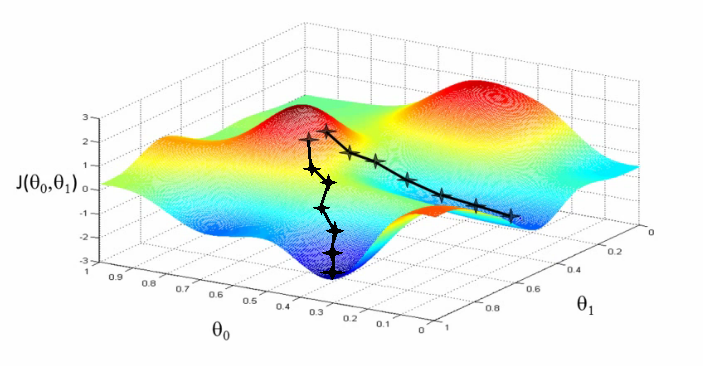
\includegraphics[width=\textwidth]{img/grad_desc.png}
\caption{Descentes de gradient avec deux initialisations différentes}
\label{fig:grad_desc}
\end{figure}


\subsection{Rétropropagation de gradient}
La \emph{rétropropagation de gradient}, (\emph{gradient backpropagation} en anglais) redonna un souffle de vie aux réseaux de neurones, lesquels résistaient à toutes les tentatives pour les entraîner convenablement. Son principe est très simple, même si la mise en œuvre requiert un peu de réflexion.

L'idée est la suivante : dans un réseau de neurones, chaque neurone prend en entrée la sortie d'autres multiples neurones, donc sa propre sortie en dépend. Ainsi, toute erreur de sortie du réseau est imputable non seulement à la couche de sortie mais à tous les neurones du réseau. Cependant, la responsabilité dans cette erreur n'est pas équitablement partagée. Il faut alors déterminer assez précisément la contribution de chaque neurone à la réponse obtenue en sortie, et propager le résultat vers l'"arrière", à travers les couches de neurones, c'est-à-dire vers la couche d'entrée. 

Il est donc clair que la sortie \(o\) d'un neurone est fonction implicite des nombreux paramètres précédents. Donc La variation de l'entrée par rapport à l'un de ces paramètres \(w\) se calcule comme suit : 

\begin{equation}\label{eq:deriv_compos}
\frac{\partial o}{\partial w} = \frac{\partial o}{\partial \alpha} \frac{\partial \alpha}{\partial w}
\end{equation}
où \(\alpha\) est un autre paramètre quelconque dont dépend \(o\).

L'intérêt de l'expliciter, et notamment en insérant tous les paramètres intermédiaires, est que les calculs sont alors immédiats : la variation de la sortie de chaque neurone est directement calculée par rapport à la variation des paramètres de ce même neurone.

Considérons deux neurones, à une seule entrée, le second étant connecté à la sortie du premier. La règle explicitée ci-dessus stipule que la variation de la sortie \(\hat{y} = o_2 = f(w_2 o_1 + b_2) = \phi(z_2)\) (on rappelle que \(\phi\) est la fonction d'activation du neurone) par rapport à celle du poids \(w_1\) vaut : 

\begin{align*}
\frac{\partial o_2}{\partial w_1} &= \frac{\partial o_2}{\partial z_2} \frac{\partial z_2}{\partial o_1} \frac{\partial o_1}{\partial z_1} \frac{\partial z_1}{\partial w_1}\\
&= \phi'(z_2) \times w_2 \times \phi'(z_1) \times x_1
\end{align*}

De même, la variation de la sortie par rapport au biais du premier neurone vaut : 

\begin{align*}
\frac{\partial o_2}{\partial b_1} &= \frac{\partial o_2}{\partial z_2} \frac{\partial z_2}{\partial _1} \frac{\partial o_1}{\partial z_1} \frac{\partial z_1}{\partial w_1}\\
&= \phi'(z_2) \times w_2 \times \phi'(z_1)\\
\end{align*}

Finalement, on pourrait presque considérer que "rétropropagation" est simplement un autre terme pour désigner la dérivée des fonctions composées. Mais généralement, on considère que cela désigne le processus suivant, pour chaque observation d'un jeu de données :
\begin{enumerate}
\item Propagation avant : calcul de la sortie \(\hat{y}\) grâce aux paramètres du réseau
\item Calcul du coût \(\kappa(y, \hat{y})\)
\item Rétropropagation de l'erreur et des contributions 
\item Mise à jour des paramètres dans toutes les couches par une itération de la descente de gradient
\end{enumerate}

Une variante appliquée en pratique calcule d'abord les erreurs pour tous les échantillons sans mettre à jour les poids (on additionne les erreurs) et lorsque l'ensemble des données est passé une fois dans le réseau, on applique la rétropropagation en utilisant l'erreur totale. Cette méthode s'appelle entraînement par \emph{mini-lots} (\emph{mini-batch training} en anglais), et offre de meilleurs temps d'exécution.


\section{Tests}
La phase de tests est celle durant laquelle on effectue le moins de changements sur les paramètres du modèle ou les hyperparamètres. Toutefois, elle est cruciale pour déceler les défauts d'ajustement, à savoir le sous-apprentissage et le sur-apprentissage. Pour ce faire, on étudie les \emph{courbes d'apprentissage}, qui sont la représentation graphique de la fonction de coût sur les données d'entraînement et les données de test. Un exemple fictif de ces courbes est donnée par la figure \ref{fig:courbes_apprent}. 

\begin{figure}[H]
\centering
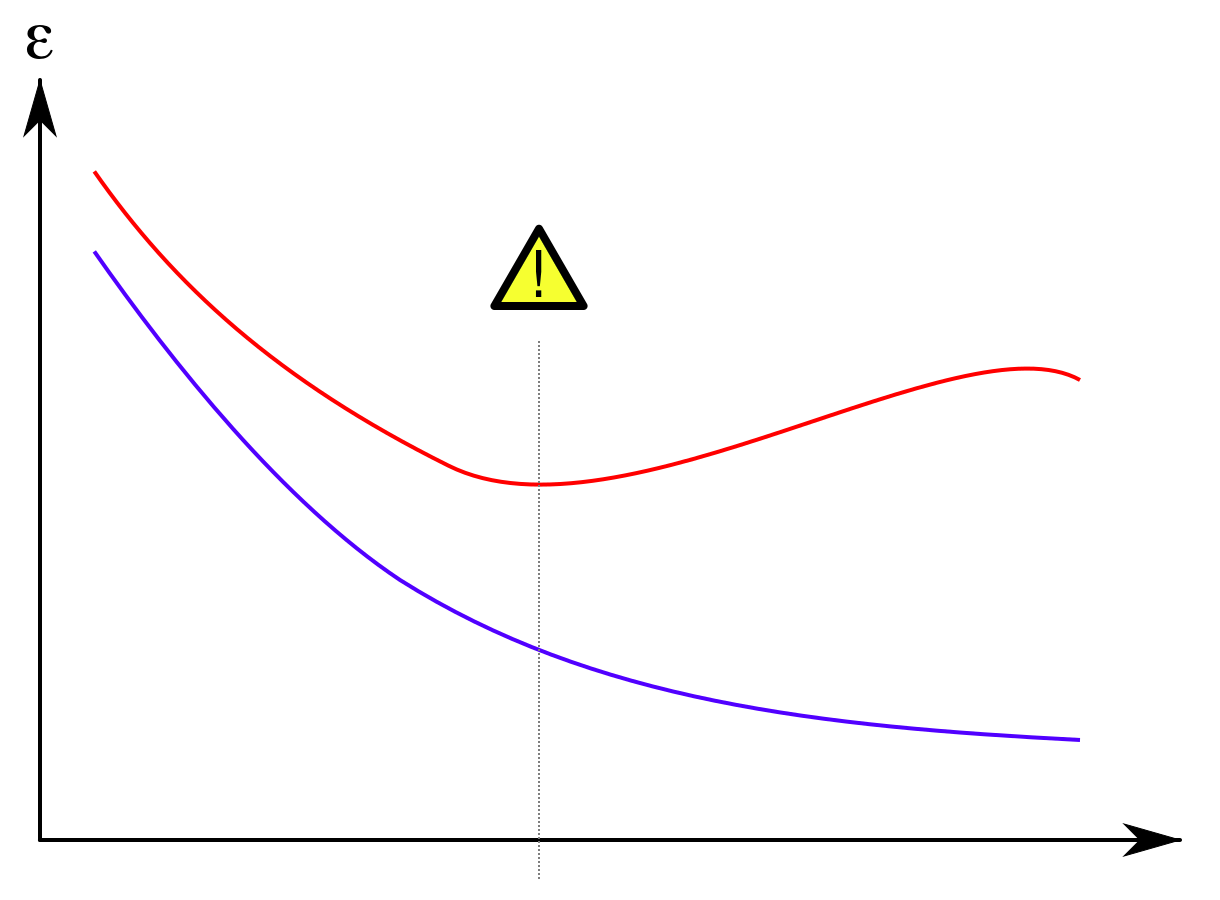
\includegraphics[width=.5\textwidth]{img/courbes_apprent.png}
\caption{Courbes d'apprentissage}
\label{fig:courbes_apprent}
\end{figure}

L'interprétation est parfois subtile mais se fait généralement comme suit. Supposons qu'à la fin de chaque phase, les deux valeurs se soient stabilisées. Si les valeurs sont toutes les deux "hautes", on est confronté à du sous-apprentissage : le modèle est peu adapté dans tous les cas. Si les deux valeurs sont "éloignées" l'une de l'autre, c'est un signe de sur-apprentissage : le modèle fait bien sur les données d'entraînement mais généralise mal.
Dans le cas où au moins une des valeurs n'est pas stabilisée : si elle fluctue avec une tendance à la baisse, il suffit de rajouter des observations. Si sa valeur augmente à nouveau, on risque le sur-apprentisage; il faut revoir le modèle.

Pour la phase de tests, il est évident qu'on doit instaurer une métrique de performances du réseau de neurones, alors que cela n'était pas si flagrant pour la première phase. De manière assez étonnante, on peut utiliser plusieurs indicateurs, donc pas uniquement la fonction de coût, pour évaluer le réseau sur des données de test. En fait, il serait même assez mal venu de se contenter de la fonction de coût pour la phase de tests. Prenons l'exemple d'un réseau résolvant un problème de classification binaire, comme celui de savoir si un texte a été écrit par Balzac ou non. Alors, on aimerait connaître les taux suivants :

\begin{description}
\item[Vrais positifs] Textes de Balzac reconnus comme tels.
\item[Vrais négatifs] Textes d'autres auteurs et catégorisés "autres"
\item[Faux positifs] Textes attribués à Balzac mais à tort
\item[Faux négatifs] Textes de Balzac non reconnus comme tels
\end{description}

La phase de tests est la plus courte en terme de temps machine, mais sans doute la plus riche en interprétations.

\section{Validation et ajustement d'hyperparamètres}
Une dernière étape pour construire un modèle satisfaisant serait de simplement en comparer plusieurs et de sélectionner le meilleur (selon la métrique de la phase de tests). On pourrait faire de petits ou bien de gros changements dans les hyperparamètres de chaque algorithme puis les tester sur des données différentes de celles d'entraînement, appelées jeu de \emph{validation}.

Pour ce faire, on pourrait diviser le jeu de données initial en 3 : entraînement (60\%), tests (20\%), validation (20\%). Ceci est envisageable avec des jeux de données immenses, pour lesquels réserver 40\% n'est pas délétère. Mais il existe un moyen élégant de s'en passer, appelé \emph{validation croisée}. Plutôt que de réserver des données uniquement pour la validation, on découpe les données en \(k\) morceaux. On choisit alors un modèle et des hyperparamètres de l'algorithme. Ensuite, on entraîne le modèle sur tous les morceaux sauf le premier; ce dernier sert à évaluer le modèle. On réinitialise ce modèle (on en efface les paramètres appris), puis on l'entraîne sur tous les morceaux sauf le second, qui, encore une fois, sert à évaluer le modèle. En répétant ce processus pour les \(k\) morceaux, on peut obtenir tout autant d'évaluations pour une combinaison d'hyperparamètres; avec la validation classique, on aurait testé les hyperparamètres une seule fois (plus exactement sur un seul jeu de données) avant d'en choisir d'autres.

Bien sûr, même si on a la possibilité de changer les valeurs des hyperparamètres, on ne sait pas nécessairement quelle valeur leur donner. On a développé des techniques pour ce cas, mais en principe, optimiser des hyperparamètres est un problème d'optimisation classique. On citera donc comme techniques la recherche aléatoire, la recherche sur grille, l'optimisation évolutionniste et même la descente de gradient !

Voici quelques exemples d'hyperparamètres que l'on change en espérant améliorer les résultats de l'algorithme.

\subsection{Taux d'apprentissage}
Comme on l'a vu, le taux d'apprentissage \(\eta\) sert à contrôler le pas de descente de gradient. Or, en le gardant constant, on risque fort de manquer le minimum (local ou global) de la fonction de coût. S'il est trop faible, l'apprentissage est trop long, et la descente de gradient pourrait s'arrêter prématurément. En revanche, s'il est trop élevé, la descente de gradient pourrait diverger ! En voici plusieurs illustrations (figure \ref{fig:taux_apprent}).

\begin{figure}[H]
\centering
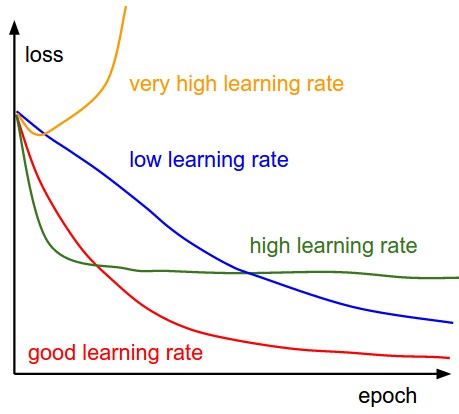
\includegraphics[width=0.65\textwidth]{img/taux_apprent.png}
\caption{Influence du taux d'apprentissage sur la fonction de coût}
\label{fig:taux_apprent}
\end{figure}

Pour remédier à cela, on dispose de plusieurs solutions. La plus facile conceptuellement consiste à diminuer le taux d'apprentissage au fur et à mesure des itérations. Dans ce cas, les premières itérations provoqueront de grands changements dans les paramètres, mais les dernières ne feront que peaufiner ces changements.

Autrement, on envisage aussi l'a version "avec inertie", dont l'objectif est de sortir des minima locaux. Les détails importent peu ici, on peut se contenter d'imaginer un ballon roulant sur une pente et prenant de la vitesse.

\subsection{Fonction d'activation}
Comme on a pu s'en apercevoir, les fonctions d'activation sont nombreuses et vairées. D'expérience, les chercheurs savent quelle fonction d'activation employer selon la place d'un neurone dans le réseau ou selon le type de problème résolu. Ainsi, la plupart du temps, les neurones de la couche de sortie peuvent avoir une fonction d'activation différente selon que le réseau réalise une classification ou une régression.

Au début des neurones non linéaires, la fonction sigmoïde \(sigma : t \mapsto \frac{1}{1 + e^{-t}}\) fut beaucoup utilisée. Cependant, ses propriétés ne sont pas restées intéressantes indéfiniment. On a donc cherché des fonctions non saturantes et facilitant l'apprentissage, telles que \(\mathit{ReLU} : t \mapsto max(0, t)\).

Assez vite, on a élaboré des variations d'après ReLU, comme "leaky ReLU" ou "parametric ReLU" (\(\mathit{PReLU} : t \mapsto max(t, \alpha t)\)), où \(\alpha\) est, étrangement, un paramètre appris en même temps que tous les paramètres. Parfois, la frontière entre paramètre du modèle et paramètre de l'algorithme est brouillée. Il n'en demeure pas moins que la fonction d'activation est considérée comme un hyperparamètre.

\subsection{Taille du réseau de neurones}
La taille d'un réseau de neurones a un impact flagrant sur les performances de celui-ci, tant en terme de temps machine qu'en terme de précision dans ses prédictions. Un grand réseau peut à la fois être très lent à entraîner et sur-ajuster les données. D'une certaine manière, plus on a de neurones dans le réseau, plus on risque de mal apprendre, mais ne pas en avoir assez n'est pas idéal non plus; le nombre de paramètres du modèle est donc un hyperparamètre de l'algorithme.

De manière assez remarquable, il existe un compromis entre mettre en place un gros réseau et un réseau plus modeste : il s'agit du \emph{décrochage} (\emph{dropout} en anglais). Il s'agit simplement, pendant l'apprentissage, de virtuellement considérer comme absents certains neurones du réseau.

Plus généralement, cette technique fait partie des méthodes de \emph{régularisation}, dont le but est de pénaliser les modèles complexes au profit des plus simples. Cela peut se traduire par exemple en ajoutant une valeur maximale aux paramètres du modèle. Encore une fois, l'idée est de réduire du mieux possible le sur-ajustement